\documentclass[addpoints]{exam}
\usepackage{cmbright}
\usepackage{amsmath}
\usepackage{amssymb}
\usepackage{graphicx}
\usepackage{mhchem}
\setlength\fillinlinelength{2em}

\header{CHE 525: math for CBEE's}{homework \#2}{fall 2025}

\begin{document}

do all of these questions by hand, i.e. without a computer. of course, check your answers with Julia.

\begin{questions}
\subsection*{matrix times vector}
%\question consider the following system of equations:
%\begin{align*}
%	x+y+z&=2 \\
%	x+2y+z&=3 \\
%	2x+3y+2z&=5.
%\end{align*}
%note, the first equation plus the second equation equals the third equation.
%each equation describes a plane in a 3D space.
%the first two planes meet along a line. the third plane contains that line, because if $x$, $y$, $z$ satisfy the first two equations then they also satisfy \fillin. these equations have infinitely many solutions (a whole line $L$). find three solutions on that line $L$. 
%
%\question move the third plane in problem \#1 to a parallel plane $2x+3y+2z=9$. now, the system has no solution. why not? the first two planes meet along the line $L$, but the third plane doesn't \fillin that line.
%
%\question in problem \#1, the columns of $A$ in the problem $A\mathbf{x}=\mathbf{b}$ are $[1, 1, 2]$, $[1, 2, 3]$, and $[1, 1, 2]$. this is a ``singular'' case because the third column is \fillin. find two combinations of the columns that give $\mathbf{b}=[2, 3,5]$. this is only possible for $\mathbf{b}=[4, 6,c]$ for what value of $c$?

\question compute $A \mathbf{x}$ by dot products of the rows with the column vector. repeat, but now as a combination of the columns of $A$. 
\begin{equation*}
	\begin{bmatrix}
	1 & 2 & 4 \\
	-2 & 3 & 1 \\
	-4 & 1 & 2
	\end{bmatrix}
	\begin{bmatrix}
	 2 \\
	 2 \\
	 3
	\end{bmatrix}
\end{equation*}
(the two methods should give consistent results.)

\question multiply $A$ times $\mathbf{x}$ to find the three components of $A\mathbf{x}$, for the two systems below.
\begin{equation*}
	\begin{bmatrix}
	0 & 0 & 1 \\
	0 & 1 & 0 \\
	1 & 0 & 0
	\end{bmatrix}
	\begin{bmatrix}
	 x \\
	 y \\
	 z
	\end{bmatrix}
\end{equation*}
\begin{equation*}
	\begin{bmatrix}
	2 & 1  \\
	1 & 2 \\
	3 & 3
	\end{bmatrix}
	\begin{bmatrix}
	 1 \\
	 1
	\end{bmatrix}
\end{equation*}

\question
\begin{parts}
	\part what 2 by 2 matrix $R$ rotates every vector by 90$^\circ$?
	
\begin{equation*}
	R
	\begin{bmatrix}
	 x \\
	 y
	\end{bmatrix}
	=
	\begin{bmatrix}
	 y \\
	 -x
	\end{bmatrix}
\end{equation*}
(sketch out the two vectors to see this transformation does this rotation.)

\part what 2 by 2 matrix $R^2$ rotates every vector by 180$^\circ$?
	
\end{parts}

\question what 3 by 3 matrix $E$ multiplies $[x, y, z]$ to give $[x, y, z+x]$?
what matrix $E^{-1}$ multiplies $[x, y, z]$ to give $[x, y, z-x]$?

\question what 2 by 2 matrix $P_1$ projects the vector $[x, y]$ onto the $x$-axis to produce $[x,0]$?

\question what 2 by 2 matrix $R$ rotates every vector through 45$^\circ$? 
\begin{equation*}
	R
	\begin{bmatrix}
	 1 \\
	 0
	\end{bmatrix}
	=
	?
\end{equation*}

\begin{equation*}
	R
	\begin{bmatrix}
	 0 \\
	 1
	\end{bmatrix}
	=
	?
\end{equation*}
so $R=?$

\question draw the row and column pictures for the equations $x-2y=0$ and $x+y=6$.

\question a 9 by 9 Sudoku matrix $S$ has the numbers 1, ..., 9 in every row and every column (in different order). for the all ones vector $\mathbf{x}=[1, ..., 1]$, what is $S\mathbf{x}$?

\subsection*{elimination [of unknowns in a linear system of equations]}
\question apply elimination and back substitution to solve:
\begin{align*}
	2x-3y &=3 \\
	4x-5y+z&=7 \\
	2x-y-3z&=5.
\end{align*}
list the three row operations in the form ``subtract \fillin times row \fillin from row \fillin''.

\question what number $d$ forces a row exchange, and what is the triangular system (not singular) for that $d$? which $d$ makes this system singular?
\begin{align*}
	2x+5y+z &=0 \\
	4x+dy+z&=2 \\
	y-z&=3.
\end{align*}

\question what number $q$ makes this system singular and which right side $t$ gives it infinitely many solutions?
\begin{align*}
	x+4y-2z &=1 \\
	x+7y-6z&=6 \\
	3y+qz&=t.
\end{align*}

\question what three matrices $E_1$, $E_2$, $E_3$ put $A$ into upper-triangular form $U$ i.e. $U=E_3E_2E_1 A$? 

\begin{equation*}
	A=\begin{bmatrix}
	1 & 1 & 0  \\
	4 & 6 & 1 \\
	-2 & 2 & 0 
	\end{bmatrix}
\end{equation*}

\question include $\mathbf{b}=[1, 0, 0]$ as a fourth column in the previous problem to produce $[A \quad \mathbf{b}]$. carry out the elimination steps on this augmented matrix to solve $A\mathbf{x}=\mathbf{b}$.

\question apply elimination to the 3 by 4 augmented matrix $[A \quad \mathbf{b}]$. how do you know this system has no solution? change the last number 6 so there \emph{is} a solution.
\begin{equation*}
	\begin{bmatrix}
	1 & 2 & 3  \\
	2 & 3 & 4 \\
	3 & 5 & 7
	\end{bmatrix}
	\begin{bmatrix}
	 x \\
	 y\\
	 z
	\end{bmatrix}
	= 
	\begin{bmatrix}
	 1 \\
	 2 \\
	 6
	\end{bmatrix}
\end{equation*}

%\question is $(A+B)^2$ different from $A+2AB + B^2$? test with these two matrices. compute by hand.
%\begin{equation*}
%	A = \begin{bmatrix}
%	1 & 2  \\
%	0 & 0 
%	\end{bmatrix}
%	\quad \quad
%	B = \begin{bmatrix}
%	1 & 0  \\
%	3 & 0 
%	\end{bmatrix}
%\end{equation*}

\subsection*{matrix times matrix}
\question multiply $AB$ using columns times rows:
\begin{equation*}
	\begin{bmatrix}
	1 & 0  \\
	2 & 4 \\
	2 & 1
	\end{bmatrix}
	\begin{bmatrix}
	3 & 3 & 0  \\
	1 & 2 & 1 
	\end{bmatrix}
\end{equation*}

\question consider the undirected graph below. write its adjacency matrix $S$. compute $S^4$ via Julia. using $S^4$, determine how many walks of length 4 exist from node 2 to node 4. sketch all of these walks.

\begin{center}
	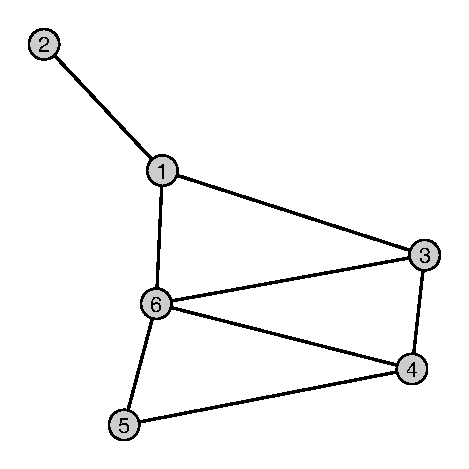
\includegraphics[width=0.5\linewidth]{my_graph.pdf}
\end{center}

\subsection*{matrix inverse}

\question compute $A^{-1}$ by setting up two systems of equations and solving both.
\begin{equation*}
	A = \begin{bmatrix}
	10 & 20  \\
	20 & 50 
	\end{bmatrix}
\end{equation*}

\question compute $A^{-1}$ by Gauss-Jordan elimination on $[A \quad \mathbf{b}]$.
\begin{equation*}
	A = \begin{bmatrix}
	1 & 3  \\
	2 & 7 
	\end{bmatrix}
\end{equation*}

\subsection*{$A=LU$ factorization}

\question what matrix $E$ puts $A$ into upper-triangular form $U=EA$? multiply by $E^{-1}=L$ to factor $A$ into $LU$.
\begin{equation*}
	\begin{bmatrix}
	2 & 1 & 0  \\
	0 & 4 & 2 \\
	6 & 3 & 5
	\end{bmatrix}
\end{equation*}

\question what matrix $E$ puts $A$ into upper-triangular form $U=EA$? multiply by $E^{-1}=L$ to factor $A$ into $LU$.
\begin{equation*}
	\begin{bmatrix}
	2 & 1 & 0  \\
	0 & 4 & 2 \\
	6 & 3 & 5
	\end{bmatrix}
\end{equation*}

\question (spend the most time understanding this one...) solve the following system $A\mathbf{x}=\mathbf{b}$ for $\mathbf{x}$ via (1) factoring $A=LU$ then (2) solving (a) the lower triangular system $L\mathbf{c}=\mathbf{b}$ followed by the upper triangular system $U\mathbf{x}=\mathbf{b}$. this is how computers solve linear systems of equations!

\end{questions}

 (\emph{source} for linear algebra problems: ``Introduction to Linear Algebra'' by Strang, 5th Ed., 2016)
\end{document}
